\documentclass[paper=a4, fontsize=11pt]{scrartcl}
\usepackage[a4paper, top=3cm, left=3cm, bottom=2cm, right=2cm]{geometry}
\usepackage[portuguese]{babel}
\usepackage[utf8]{inputenc}
\usepackage{amsmath,amsfonts,amsthm,amssymb}
\usepackage{sectsty}
\usepackage{enumerate}
\allsectionsfont{\normalfont\scshape}
\newcommand{\horrule}[1]{\rule{\linewidth}{#1}}
\usepackage{natbib}
\usepackage[dvipsnames]{xcolor}
\usepackage{graphicx}

\newcommand{\comment}[1]{}

\definecolor{VioletRed4}{RGB}{139 ,034 ,082}

\begin{document}

\normalfont \normalsize 
\hspace{2.3cm} \textsc{universidade federal de Minas Gerais -- Eduarda Chagas}\\[25pt]
\horrule{0.5pt} \\[0.5cm]
\indent \huge Revisão sistemática -- SAR em Computação Urbana\\ 
\horrule{2pt} \\[0.5cm]
\normalfont \normalsize 
%---------------------------------------------------------------------------------------------
\comment{
\section*{1 -- A Review of PolSAR Image Classification: From Polarimetry to Deep Learning}

This paper presents a review of the classification techniques of terrain regions.

\begin{itemize}
    \item Autores:~\cite{Wang2019Review}
    \item Data de publicação: Aug. 2019
    \item Técnica utilizada: The network structure and training algorithm of real-valued convolutional neural network (RV-CNN) and complex-valued neural network (CV-NN).
    \item Foco do artigo: In this paper, the neural network algorithm and PolSAR data characteristics are combined and studied to improve the performance of terrain classification.
\end{itemize}

\newpage
}

\section*{An entropy-based classification scheme for land applications of polarimetric SAR data}

The alpha-entropy approach is based on the eigenvector analysis of the coherency matrix, where the alpha angle is related to the target scattering type with $0^0 < alpha < 90^0$ and the entropy describes the randomness of a scattering process. 

Since the alpha angle and entropy describe the scattering mechanism, this approach can be used in classification of targets based on different scattering mechanisms. 
The H/Alpha plane is often used for image classification.

\begin{itemize}
    \item Autores:~\cite{cloude1997entropy}
    \item Data de publicação: Jan 1997
    \item Dataset
    \begin{itemize}
        \item Fonte: ASA/JPL AIRSAR data base.
        \item Região analisada: L-Band data for the San Francisco mixed urban/vegetation/ocean scene and two frequency (P and C-Band) data for the Landes forest in south-west France.
    \end{itemize}
    \item Estruturas de dados: we generally have access either to complete coherent scattering matrix data or to multilook averaged Stokes matrix data. In either case, we can form local estimates of the coherency matrix using pixel averaging.
    \item Técnica utilizada: unsupervised $H-\alpha$ method uses these two parameters to describe the entropy and scattering mechanism types, where scatterers are classified in the $H/\alpha$ plane into eight zones. The method relies on an eigenvalue analysis of the coherency matrix and employs a three-level Bernoulli statistical model to generate estimates of the average target scattering matrix parameters from the data.
    \item Técnicas de visualização dos dados: Shows the nine-zone classification results in a color coded format.
    \item Validação dos resultados: Dataset.
    \item Foco do artigo: classifier has correctly identified the key physical features of this scene such as the sea surface, the coastal zone, the urban areas (with moderate entropy dihedral scattering) and finally the vegetated areas 
    \item Desafios e trabalhos futuros: It is our aim to next extend this classification scheme into inversion, based on physical and scattering models for surface and volume features.
\end{itemize}

\newpage

\section*{Urban Area Mapping from Polarimetric SAR data using Fuzzy Inference System}

In particular, our aim is to utilize the profound knowledge available about scattering mechanism from urban targets to delineate urban environment. 
In this approach, we have utilized the recently developed polarimetric SAR scattering power decomposition technique (SD-Y4O) given in Bhattacharya.

In this study, we have used full polarimetric SAR data for urban area mapping using a fuzzy inference system.
This has been motivated by the fact that well documented knowledge regarding scattering mechanisms usually present in urban area is available. 
This knowledge is incorporated in forming the rules of the fuzzy inference system used to determine urban areas present in a PolSAR image.

Pre-processing of data is necessary to get the inputs of the fuzzy inference system. 
Coherency matrix is obtained by multi-looking the PolSAR data. 
Lee filtering is used to further smoothen it and remove speckle noise.
Scattering powers are computed over a $7 \times 7$ window, using the modified target decomposition algorithm. 
Double bounce (Pd), surface scattering (Ps), volume scattering (Pv) and helical scattering (Ph) are estimated along with the polarization orientation angle whose standard deviation is also calculated. 
Span which gives the total intensity is computed by summing up the scattering powers. 
The magnitude of the correlation between the HV and HH-HV component is obtained from $T_{23}$ element of the coherency matrix.
To define appropriate fuzzy membership functions for each of the inputs, normalization is done as shown in Fig.~\ref{Fig:pre-processing}. 
The histogram of each of the inputs is first equalized and then an inverse cumulative distribution function of the Gaussian distribution is applied. 

\begin{figure}[hbt]
	\centering
	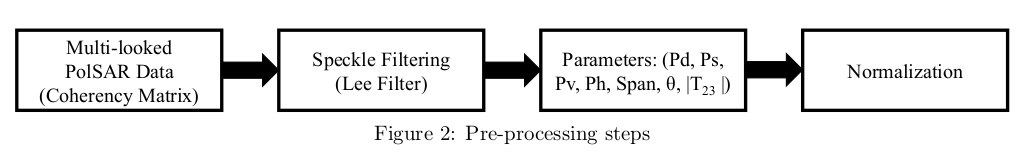
\includegraphics[width=0.7\linewidth]{Figures/Pre-processing.jpg}
	\label{Fig:pre-processing}
\end{figure}

\begin{itemize}
    \item Autores:~\cite{ahluwalia2016urban}
    \item Data de publicação: May. 2016
    \item Dataset
    \begin{itemize}
        \item Fonte: ALOS PALSAR L-band polarimetric SAR.
        \item Tempo de coleta: 27th November 2009
        \item Região analisada: Data acquired over Chennai, Tamilnadu, India.
    \end{itemize}
    \item Estruturas de dados: Coherency Matrix.
    \item Técnica utilizada: Fuzzy inference system (FIS) and k-means clustering.
    \item Técnicas de visualização dos dados: The Pauli RGB image of the study area along with the optical image.
    \item Validação dos resultados: Dataset.
    \item Foco do artigo: Urban area mapping from full-polarimetric synthetic aperture radar (SAR) data.
    \item Desafios e trabalhos futuros: A defined method to find the value of number of desired clusters (N) that gives a suitable result will be looked upon in our future work.
\end{itemize}

\newpage

\section*{Urban Area Extraction in SAR Data}

For a better discrimination, all texture measures are calculated and a PCA rotation is applied to them and the first PC is multiplied by the urban inhomogeneity parameter and the obtained image is segmented. 
The obtained results of this procedure comparing with the K-Means clustering algorithm show the better performance of this algorithm for urban area detection.

FFMAX -- This method that is mostly a descriptor for urban areas, assume that the amplitude image, takes value from $[0, g-1]$ where g is the maximum gray level of SAR amplitude image.
Then the algorithm uses threshold s, $s \in [0, g- 1]$ to cut the local histogram (on $60 \times 60$ window). 
Then the probability of the higher part is calculated and compared to the highest statistical frequency of the lower part.
When the first is greater than the second the central pixel receives the value of s as its current value or the value should be decreased.
This process iterates for all pixels.

Local Indicator of Spatial Association (LISA) -- are local indicators of spatial autocorrelation, which are widely used in GIS studies. Evaluate the similarity between the neighbours of a pixel by comparing its value with average local value.

Square Root Pair Difference (SRPD) -- is a semi-variogram texture measure.

Wavelet texture Measure and finally Fractal Dimension.

After applying PCA, its first component is multiplied by a man-made structure highlighting parameter. 
The reason of using the first PC is that it is well-known that this PC has the highest level of spatial information in comparison to the rest of them. Finally, by segmenting this image, the urban areas are extracted.

\begin{itemize}
    \item Autores:~\cite{aghababaee2013urban}
    \item Data de publicação: Oct. 2013
    \item Dataset
    \begin{itemize}
        \item Fonte: TerraSAR-X
        \item Região analisada: urban area in Japan.
    \end{itemize}
    \item Redução de dimensionalidade: textures measures are calculated.
    \item Estruturas de dados: Scattering matrix.
    \item Técnica utilizada:  The textures are extracted from the amplitude images. Then a simple and powerful estimator called inhomogeneity parameter for the urban structures highlighting is computed and multiplied by the first component of PCA. Finally the urban areas are extracted from the multiplied image using a binary decision method. 
    \item Técnicas de visualização dos dados: textures.
    \item Validação dos resultados: Dataset
    \item Foco do artigo: In this paper, the performance of different texture measures for detection of urban areas from SAR data is evaluated.
    \item Desafios e trabalhos futuros: However, the framework needs to be applied to an enormous SAR image database and also to the different SAR sensors image.
\end{itemize}

\newpage

\section*{Urban Extraction from SAR Images Using Local Statistical Characteristics and Gaussian Markov Random Field Model}

First, a probability map of the urban areas is computed based on local statistical characteristics, using an ffmax operator proposed by C. Gouinaud.
Then the Gaussian MRF model is adopted to describe the texture of urban zones and the parameters of the model are estimated from the original image together with the probability map. 
Finally, the urban areas are extracted under Bayesian framework by maximum a posterior (MAP) criterion, with modeling the urban label field by Potts model.

Such information is also used in communication management and military intelligence [1].

The flow chart of the proposed unsupervised urban extraction scheme is shown in Fig.~\ref{Fig:flow}.

\begin{figure}[hbt]
	\centering
	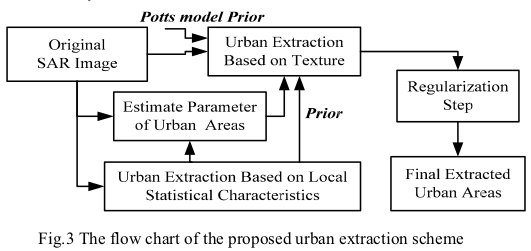
\includegraphics[width=0.7\linewidth]{Figures/flow.jpg}
	\label{Fig:flow}
\end{figure}

\begin{itemize}
    \item Autores:~\cite{xia2006urban}
    \item Data de publicação: Nov. 2006
    \item Dataset
    \begin{itemize}
        \item Fonte: ERS-1 SAR image
        \item Tempo de coleta: 1996
        \item Região analisada: Shenzhen area in China
    \end{itemize}
    \item Estruturas de dados: Texture
    \item Técnica utilizada: Local statistical characteristics and texture information described by Gaussian Markov Random Field (MRF) model.
    \item Técnicas de visualização dos dados: original 3 looks ERS-1 SAR image (with the size of $1024 \times 1280$).
    \item Validação dos resultados: The performance of the proposed method is evaluated by experimental results on real SAR images.
    \item Foco do artigo: Extract urban areas from SAR images .
    \item Desafios e trabalhos futuros: The extraction result of urban areas can be taken as a pre-classification of high level processing such as image interpretation and can be used for communication management and military intelligence. 
\end{itemize}

\newpage

\section*{Urban Areas Detection using Polarimetric SAR Images}

We computed the Yamaguchi polarimetric decomposition directly from polarimetric data without the disorientation process and by comparison to the result of decomposition with the disorientation process. 
We note that the last method is better because it allows the detection of double bounce power in the oblique urban areas.

If $(P_{double} > P_{volume} and P_{surface} > P_{volume})$ then the area is urban else the area is non-urban.


\begin{itemize}
    \item Autores:~\cite{azmedroub2015urban}
    \item Data de publicação: July 2015
    \item Dataset
    \begin{itemize}
        \item Fonte: C band by RadarSAT-2
        \item Tempo de coleta:
        \item Volume dos dados:
        \item Região analisada: city of Algiers in Algeria.
    \end{itemize}
    \item Estruturas de dados: Coherency matrix
    \item Técnica utilizada: The proposed algorithm for urban areas detection uses a comparison between the scattering powers computed from the Yamaguchi four components decomposition as a condition to discriminate data in urban and non-urban. Then we use the maximum likelihood complex Wishart classifier to improve the result.
    \item Técnicas de visualização dos dados: RGB of Yamaguchi decomposition and Google earth image of the selected region
    \item Validação dos resultados: The result is very accurate in comparison to the optical image extracted from Google earth.
    \item Foco do artigo: Algorithm for urban areas detection.
    \item Desafios e trabalhos futuros: Many further analyses are needed to discriminate between different types of urban areas as well as the application to other PolSAR data.
\end{itemize}

\newpage

\section*{Urban Boundary Extraction Using 2-component Polarimetric SAR Decomposition}

\begin{itemize}
    \item Autores:~\cite{storie2012urban}
    \item Data de publicação: July 2015
    \item Dataset
    \begin{itemize}
        \item Fonte: Multitemporal, fully polarimetric RADARSAT 2 fine beam SAR imagery. All data were acquired in quad-polarization mode (HH-HV-VH-VV) with an incidence angle of $37.38^0$ to $38.89^0$ (FQ18). All images have a fine spatial resolution ($12m$ range $\times 8m$ azimuth) acquired from an altitude of 750 kilometers. RADARSAT-2 data is acquired in C-band (5.4 cm wavelength) and is processed at 32-bit radiometric resolution.
        \item Tempo de coleta: Acquired for July 29, 2009 and July 24, 2010.
        \item Região analisada: City of San Juan, Argentina and its surrounding rural areas.
    \end{itemize}
    \item Estruturas de dados: Complex scattering matrix.
    \item Técnica utilizada: Neumann 2-Component decomposition.
    \item Técnicas de visualização dos dados: PauliRGB and 2-Component Decompositions: a) Barnes (T22), b) Holm (T22), c) Freeman (Ground dB), d) Neumann (Delta).
    \item Validação dos resultados: Dataset.
    \item Foco do artigo: This research investigates the capability of using multitemporal, fully polarimetric RADARSAT fine beam SAR imagery for urban boundary mapping and change detection.
    \item Desafios e trabalhos futuros: Future research will apply this technique as part of larger project that seeks to quantify, based upon multiple scattering mechanisms, the transition zone between the urban and rural environments with the goal of creating a three category classification (urban, transition, rural) for the purposes of long-term urban monitoring and mapping. The identification of rapidly urbanized or expanding urban areas is a critical first step in the long-term monitoring and sustainable planning of the overall urban system.
\end{itemize}

\newpage

\section*{Urban Area Man-Made Target Detection for PolSAR Data Based on a Nonzero-Mean Statistical Model}

The likelihood ratio is a ratio of the likelihood function varying the parameters over two distinct sets in the numerator and denominator [17]. 
The generalized likelihood ratio test (GLRT) is a statistical test for making a decision between two hypotheses based on the value of this ratio.

The targets are categorized into five classes: large building, small building, large natural surface, small areas of grass, and bare soil.

The results obtained by PMZM based on the Wishart distribution and SMNM based on the Rician distribution are shown.
The coherence or co-variance matrix is calculated by averaging the information of all the pixels in a moving window. 
Thus, the resolution is reduced during the process.

SMNM achieves excellent overall accuracy in man-made target detection and poor accuracy in natural target detection.
In contrast, the proposed method achieves high accuracy for natural target detection. 
The performance for large buildings is also satisfactory. 
However, the detection accuracy for small houses, which is less nonstationary than that for large buildings, is about $14\%$ lower than SMNM. 
This indicates that the new method tends to recognize targets as natural ones, which will cause missed detection.

\begin{itemize}
    \item Autores:~\cite{wu2014urban}
    \item Data de publicação: April 2014
    \item Dataset
    \begin{itemize}
        \item Fonte: E-SAR data with HH, HV, VH, and VV channels were used in the experiments. E-SAR is an airborne SAR system owned by the German Aerospace Center (DLR). The full-polarization mode is in the L-band with a spatial resolution of about $3m$ in both the azimuth and range direction. The azimuth beamwidth is $18^0$[19], which is large enough to grant proper azimuth stationarity extraction.
        \item Região analisada: Dresden, Germany.
    \end{itemize}
    \item Estruturas de dados: Statistical Model: scattering matrix.
    \item Técnica utilizada: The method involves two main steps, which include generating sub-aperture images by implementing the azimuth time–frequency decomposition and examining the azimuth stationarity via GLRT.
    \item Técnicas de visualização dos dados: Optical image obtained from Google Earth and the Pauli basis PolSAR image that shows double-bounce scatterings in the red channel, volume scatterings in the green channel, and surface scatterings in the blue channel.
    \item Validação dos resultados: Pauli basis.
    \item Foco do artigo: Man-made target detection using synthetic aperture radar (SAR).
\end{itemize}

\newpage

\section*{Discrimination of forests and man-made targets in SAR images based on spectrum analysis}

\begin{itemize}
    \item Autores:~\cite{zou2019discrimination}
    \item Data de publicação: May 2019
    \item Dataset
    \begin{itemize}
        \item Fonte: E-SAR image provided by German Aerospace Centre (DLR).
        \item Região analisada: Oberpfaffenhofen in Germany.
    \end{itemize}
    \item Técnica utilizada: Spectrum analysis is employed to construct a novel method named Modified Spectrum Power. Fourier transformation.
    \item Técnicas de visualização dos dados: Optical and SAR Images.
    \item Validação dos resultados: Optical image, and the roughly labeled images.
    \item Foco do artigo: Based on the Modified Spectrum Power, forests can be discriminated from other targets with a high accuracy and man-made targets can be discriminated based on it.
\end{itemize}

\newpage

\section*{Novel Techniques for Built-Up Area Extraction from Polarimetric SAR Images}

The first method is based on the three dominant scattering types in the scene and compares them with scattering models; if any of them matches with built-up type elementary scattering models, then the pixel is said to belong to a built-up area. 
The second method is based on a novel PolSAR built-up index (RBUI) composed by considering scattering mechanisms from built-up structures.

In this study we propose a scattering similarity-based approach using the observed data and specific elementary scattering models. 
Additionally, a new radar built-up index (RBUI) is proposed and validated in two test locations with data acquired by two different PolSAR sensors.

In the radar built-up index (RBUI) maps the majority of built-up structures show a value greater than 0.5, while water bodies and bare surface have values ranging between 0 and 0.1.
The areas with vegetation fall on the lower side of 0.5. 
The flowchart of the two approaches for the extraction of a built-up area map using PolSAR data is shown in Fig.~\ref{Fig:Flowchart}.

\begin{figure}[hbt]
	\centering
	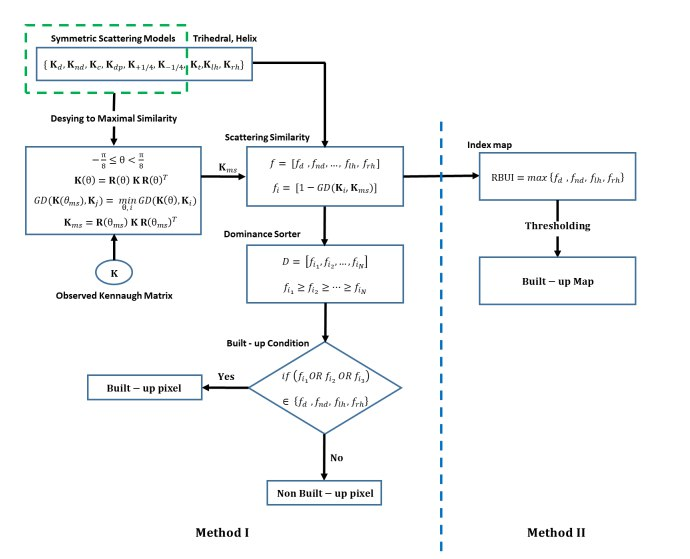
\includegraphics[width=0.5\linewidth]{Figures/Flowchart.jpg}
	\label{Fig:Flowchart}
\end{figure}

\begin{itemize}
    \item Autores:~\cite{ratha2019novel}
    \item Data de publicação: Jun. 2019
    \item Dataset
    \begin{itemize}
        \item Fonte: C-band by RADARSAT-2 and other at L-band by ALOS-2 SAR sensors. 
        %The incidence angle varies from $28.0^0$ to $29.8^0$ from near to far range for the RADARSAT-2 image, and the scene-centered incidence angle is $30.9^0$ for the ALOS-2 image. The San-Francisco image ($762 \times 978$ pixels) is multilooked by a factor of $2$ in range and $4$ in azimuth effectively providing a ground range pixel resolution of $20$m while the Kyoto image ($1616 \times 2826$ pixels) is multilooked by a factor of $3$ in range and $5$ in azimuth providing a ground range pixel resolution of $15.7$m.
        \item Região analisada: San-Francisco, USA and Kyoto, Japan.
    \end{itemize}
    \item Estruturas de dados: Scattering matrix and then Kennaugh matrix and coherency matrix.
    \item Técnica utilizada: Both methods exploit the geodesic distance on the unit sphere in the space of Kennaugh matrices.
    \item Técnicas de visualização dos dados: Pauli RGB and binary maps.
    \item Validação dos resultados: Two proposed techniques are validated on two different urban scenes. Shows the contribution of different built-up area scattering dominance types to built-up producer accuracy of methods.
    \item Foco do artigo: Propose two built-up area extraction techniques based on the analysis of fully PolSAR data.
    \item Desafios e trabalhos futuros: In the future, besides exploiting this information more extensively, we plan to extend the methodology to bistatic radar datasets.
\end{itemize}

\newpage

\section*{Online Random Forests for Urban Area Classification from Polarimetric SAR Images}

Machine-learning based approaches usually represent the neighborhood of a pixel by a set of features and thus transform low-dimensional image matrices into high-dimensional data cubes.
One solution is to limit the used data to a sufficiently small subset.
This allows to apply any of the available machine learning frameworks and train them “offline”, i.e. with access to all samples in the training subset.
However, more fine-grained modern classification problems and methods with many internal parameters (e.g. to learn features from the data) are in dire need of data and will not lead to acceptable results if provided with too few samples.
The second solution is to limit the set of processing pipelines to those that are capable of batch-processing, i.e. adjusting their internal parameters incrementally based on small chunks of data.

The area contains man made as well as natural structures.
The annotation was acquired manually and consists of five different classes: City, Road, Forest, Shrubland, and Field.

\begin{itemize}
    \item Autores:~\cite{hansch2019online}
    \item Data de publicação: May 2019.
    \item Dataset
    \begin{itemize}
        \item Fonte: E-SAR sensor (DLR, L-band). The first data set is a fully polarimetric image of $1.390 \times 6.640$ pixels. TerraSAR-X (X-band) provided by DLR. It contains $10.310 \times 11.698$ pixels.
        \item Volume dos dados: The first one a rather small PolSAR image of roughly 1M pixels. The second dataset contains roughly 120M pixels.
        \item Região analisada: Oberpfaffenhofen, Germany.
    \end{itemize}
    \item Estruturas de dados: Pixels.
    \item Técnica utilizada: Random Forests variant.
    \item Técnicas de visualização dos dados: Color representation of SAR Image, the corresponding reference data, the estimated class posterior for Urban (high probability in red, low probability in blue) and the entropy of the class posterior illustrating a high uncertainty especially in misclassified areas.
    \item Validação dos resultados: The image data was manually labelled as urban or non-urban. (overall accuracy, balanced accuracy and kappa coefficient).
    \item Foco do artigo: This paper illustrates how Random Forests can be trained by batch processing, i.e. at every iteration only a small amount of samples need to be kept in memory. The benefits of this training scheme are illustrated for the use case of urban area detection from PolSAR imagery.
\end{itemize}

\newpage

\section*{Improved Extraction of Urban Extents from ASAR Wide Swath Data}

In addition to the SAR data, the routine assumes that two additional information may be provided, namely slope values sampled to the same grid as the ASAR data, as well as the number of SAR acquisitions that are combined in each position to obtain the input data.
In case the additional information is not available, the routine will use the standard set of parameter values (called “permissive”), with an inevitable increase of false positives.

The overall structure of the algorithm is presented in the following Fig.~\ref{Fig:ExtractionRoutine}.

\begin{figure}[hbt]
	\centering
	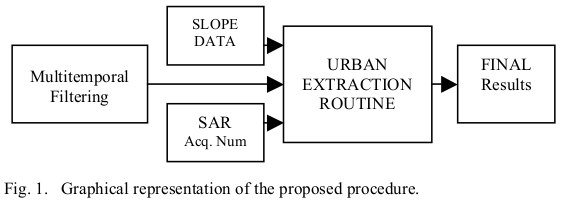
\includegraphics[width=0.7\linewidth]{Figures/ExtractionRoutine.jpg}
	\label{Fig:ExtractionRoutine}
\end{figure}

\begin{itemize}
    \item Autores:~\cite{lisini2015improved}
    \item Data de publicação: Jun. 2015
    \item Dataset
    \begin{itemize}
        \item Fonte: ASAR SWM data.
        \item Tempo de coleta: 2010
        \item Região analisada: Big cities were considered, namely Moscow, Mumbai, Paris, and Beijing. The second set of experiments was performed on a much larger area, i.e. the whole P.R. China.
    \end{itemize}
    \item Técnica utilizada: The first one estimates if any part of the extracted area falls on areas with high slopes. The second test concerns instead of false positives generated by water ruffle in the sea. 
    \item Técnicas de visualização dos dados: EO data for the same area. A comparison between the original (blue) and improved (red) urban extent extraction results (histogram). Report the same area depicted by optical sensors in Google EarthTM, for visual comparison.
    \item Validação dos resultados: For sake of comparison, the urban extent extractions were aggregated at the province level and then evaluated against the extraction performed manually by a team at Tsinghua University (P.R. China) for the most populous 663 cities of the country in the year 2010.
    \item Foco do artigo: The aim of the procedure is to generate a map of urban area extents using multi-temporal ASAR SWM data.
\end{itemize}

\newpage

\section*{Urban-Area Extraction From Polarimetric SAR Images Using Polarization Orientation Angle}

As shown in Fig.~\ref{Fig:urbanareaExtraction}, the proposed algorithm for urban-area extraction consists of two steps. 
The first step is classification of urban/mountain area and farmland/bare ground/sea. The second step then classifies the urban and mountain areas.

\begin{figure}[hbt]
	\centering
	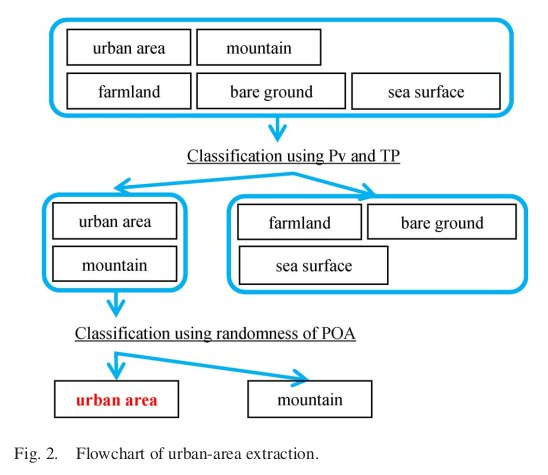
\includegraphics[width=0.4\linewidth]{Figures/urban-areaExtraction.jpg}
	\label{Fig:urbanareaExtraction}
\end{figure}

\begin{itemize}
    \item Autores:~\cite{kajimoto2012urban}
    \item Data de publicação: Aug. 2012
    \item Dataset
    \begin{itemize}
        \item Fonte: Fully polarimetric Advanced Land Observing Satellite (ALOS)/Phased-Array-type L-band SAR (PALSAR) level 1.1 data were used. 
        \item Região analisada:Three study areas were selected: Tokyo, Sapporo, and Fukuoka in Japan. Urban and farmland training data were manually selected from the Tokyo area. Thus, the threshold for discriminating between urban areas and farmland was determined for Tokyo and then optimized for other areas.
    \end{itemize}
    \item Estruturas de dados: Coherency matrix and four-component decomposition.
    \item Técnica utilizada: Polarization orientation angle (POA), volume scattering power (Pv) derived by four-component decomposition, and total power (TP).
    \item Técnicas de visualização dos dados: AVNIR-2 image and polarization orientation angle (POA) map.
    \item Validação dos resultados: Furthermore, ALOS/Advanced Visible and Near-Infrared Radiometer type 2 (AVNIR-2) optical sensor data were used as a reference.
    \item Foco do artigo: In this letter, an algorithm is proposed that robustly extracts urban areas from polarimetric synthetic aperture radar images.
\end{itemize}

\newpage

\section*{Urban Area Extraction from Polarimetric SAR Imagery Using Only Positive Samples}

\begin{itemize}
    \item Autores:~\cite{liu2010urban}
    \item Data de publicação: Dec. 2010
    \item Dataset
    \begin{itemize}
        \item Fonte: RADARSAT-2 fully PolSAR data and Radarsat-2 images.
        \item Volume dos dados: The five classes are urban area, woodland, water, mountain and cropland, separately with 392, 324, 400, 400 and 400 samples. And each
sample is an image with size $100 \times 100$ pixels.
        \item Região analisada: Flevoland and Vancouver.
    \end{itemize}
    \item Estruturas de dados: We define non-overlapping patches with $20 \times 20$ pixels for each sample image, and concatenate the feature descriptors of its 25 patches as the final feature representation.
    \item Técnica utilizada: we use a second-order GMRF, and GMRF model parameters are fitted on the span of PolSAR data.
    \item Técnicas de visualização dos dados: The original PolSAR image.
    \item Validação dos resultados: Dataset.
    \item Foco do artigo: we present a study of extracting urban areas from Polarimetric Synthetic Aperture Radar (PolSAR) images using only positive samples. We solve this problem by learning a standard binary classifier (urban/non-urban) given an incomplete set of positive samples (urban) and a set of unlabeled samples (some of which are urban and some of which are non-urban).
\end{itemize}

\newpage

\section*{Polarimetric SAR Image Classification Using Deep Convolutional Neural Networks}

RGB image, where blue, red, and green represent $T_{11}$ , $T_{22}$ , and $T_{33}$ , respectively.

The architecture of deep convolutional neural network used in this letter is shown in Fig.~\ref{Fig:Networkarchitecture}, which contains two convolution layers interleaved with two max-pooling layers, two fully connected layers, and a Softmax classifier [15] connected to the output. 
Each convolution layer is followed by a max-pooling layer, with pooling size $2 \times 2$ and a stride of 2 pixels. 
The rectified linear units (ReLU) activation function [16] is applied to the first fully connected layer.
The model was trained using back-propagation and stochastic gradient descent with minibatch size of 64 [14].

\begin{figure}[hbt]
	\centering
	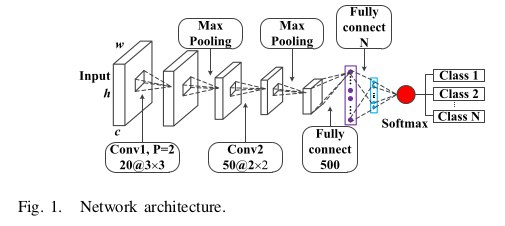
\includegraphics[width=0.7\linewidth]{Figures/Networkarchitecture.jpg}
	\label{Fig:Networkarchitecture}
\end{figure}

\begin{itemize}
    \item Autores:~\cite{zhou2016polarimetric}
    \item Data de publicação: Nov. 2016 
    \item Dataset
    \begin{itemize}
        \item Fonte: NASA/JPL AIRSAR data.
        \item Volume dos dados: The image size is $750 \times 1024$ pixels. The resolution is 6.6 m in the slant range direction and 12.1 m in the azimuth direction.
        \item Região analisada: San Francisco, CA, and Flevoland, The Netherlands.
    \end{itemize}
    \item Pré-processamento: We propose a new 6-D real vector representation tailored for neural networks.
    \item Estruturas de dados: The multi-looked POLSAR data in the format of coherency or co-variance matrix is first converted into a normalized 6-D real feature vector.
    \item Técnica utilizada: Deep convolutional neural network.
    \item Técnicas de visualização dos dados: First layer $3 \times 3$ convolution kernels learned (color coded with Pauli decomposition). Activation visualization of (a) first convolution layer and (b) second convolution layer of a rapeseed input. RGB pseudocolor image.
    \item Validação dos resultados: Compared with Google Earth optical images.
    \item Foco do artigo: This letter proposes a novel POLSAR terrain classification framework using deep convolutional neural networks.    
\end{itemize}

\newpage

\section*{A Study on Extraction of Urban Areas from Polarimetric Synthetic Aperture Radar image}

By using the polarimetric correlation coefficients in linear and circular polarization basis and the HV backscattering coefficient, a classification of urban area, vegetation area and sea area is performed. 
The algorithm of classification uses a decision tree. 
The result of classification is shown in Fig.~\ref{Fig:decisiontree}.

\begin{figure}[hbt]
	\centering
	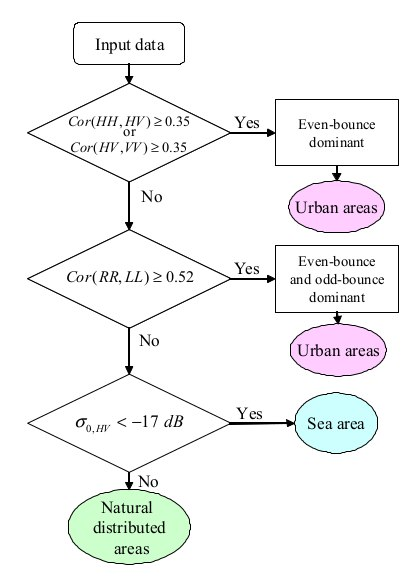
\includegraphics[width=0.3\linewidth]{Figures/decisiontree.jpg}
	\label{Fig:decisiontree}
\end{figure}


\begin{itemize}
    \item Autores:~\cite{moriyama2004study}
    \item Data de publicação: Dec. 2004
    \item Dataset
    \begin{itemize}
        \item Fonte: X-band SAR data acquired by Pi-SAR (Polarimetric and Interferometric SAR was developed by NICT and JAXA.) [6] we use only X-band data.
        \item Tempo de coleta: August 20, 2003.
        \item Volume dos dados: This image has a dimension of $4000 \times 4000$ pixels. The resolution of image is $1.5[m]$ in both the azimuth and range direction.
        \item Região analisada: Kobari area in Niigata city.
    \end{itemize}
    \item Pré-processamento: Before data analysis, the average filtering of 15 x 15 windows is applied to this polarimetric data due to the reduction of phase information dispersion.
    \item Estruturas de dados: Polarimetric scattering models and the difference of polarization basis.
    \item Técnica utilizada: Polarimetric correlation coefficient. Decision tree.
    \item Técnicas de visualização dos dados: The span image.
    \item Validação dos resultados: Dataset.
    \item Foco do artigo: In this paper, an extraction method of urban areas by the polarimetric correlation coefficient is examined. We have investigated the behavior of polarimetric correlation coefficient by using several polarimetric scattering models in the linear (HV) and the circular (RL) polarization basis [4].   
\end{itemize}

\newpage

\section*{Urban Area Detection in SAR Imagery Using a New Speckle Reduction Technique and Markov Random Field Texture Classification}

Our new filtering method is based on the spatial analysis of the detail images obtained from the wavelet decomposition of the image [2].
Each of the detail images is split into two images, each containing only the positive and the negative wavelet coefficients, respectively (the missing coefficients in each image are set to zero). 
The images are then re-scaled to the gray scale interval [0, 255]; for the negative image, this is done after taking the absolute value of each pixel. 
We call the re-scaled images the 'P' and the 'N' image, respectively.

We compare our new filter with standard speckle filters, like Lee, Frost and the gamma filter.

It is clear that our filter removes noise on all levels better than the standard filters, while preserving vital information like edges.

\begin{itemize}
    \item Autores:~\cite{Duskunovic2000urban}
    \item Data de publicação: Aug. 2002
    \item Dataset
    \begin{itemize}
        \item Fonte: SAR image of Denver.
        \item Região analisada: Denver.
    \end{itemize}
    \item Estruturas de dados: Texture.
    \item Técnica utilizada: Wavelet decomposition and Markov Random Field (MRF).
    \item Técnicas de visualização dos dados: original SAR image.
    \item Validação dos resultados: Visual analysis of noise removal.
    \item Foco do artigo: First propose a new speckle reduction method, which preserves edges and doesn’t need parameters to be adjusted, based on wavelet decomposition. Next we use the filter technique in combination with the Markov Random Field (MRF) texture classification as stated in [11] to detect urban areas in the images.
\end{itemize}

\newpage

\section*{An Adaptive and Iterative Method of Urban Area Extraction From SAR Images}

According to the statistical characteristics of urban areas, an adaptive and iterative method based on the low-level extraction given by the ffmax algorithm using a large window is proposed. 

Our method is an iterative scheme that consists of two steps: to extract urban areas using ffmax algorithm with a large fixed window and to compute the adaptive window of each pixel with local statistical characteristics. 
The Kolmogorov–Smirnov (K–S) test is used to find the adaptive window.

In this letter, square-root Gamma distribution is adopted to model SAR amplitude data.
There are several characteristics of ffmax algorithm: 1) extraction rule is robust; 2) rule not only extracts the urban zone but also permits the urban agglomeration density measures; and 3) extraction results just provide low-level description of urban zones with no precise borders.

The framework of the proposed extraction method is shown in Fig.~\ref{Fig:Framework}.

\begin{figure}[hbt]
	\centering
	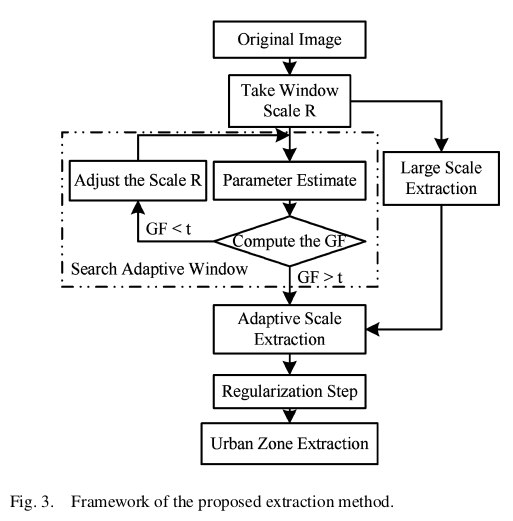
\includegraphics[width=0.5\linewidth]{Figures/Framework.jpg}
	\label{Fig:Framework}
\end{figure}

\begin{itemize}
    \item Autores:~\cite{he2006adaptive}
    \item Data de publicação: Oct. 2006
    \item Dataset
    \begin{itemize}
        \item Fonte: real SAR images.
        \item Região analisada: Matterhorn area in Switzerland.
    \end{itemize}
    \item Pré-processamento: three-look X-SAR image (with the size of $1024 \times 1024$).
    \item Técnica utilizada: Adaptive and iterative (AI) method based on ffmax algorithm.
    \item Técnicas de visualização dos dados: X-SAR image.
    \item Validação dos resultados: Dataset.
    \item Foco do artigo: This letter addresses the problem of extracting the urban areas from SAR images with high resolution.
\end{itemize}

\newpage

\section*{Statistical Analysis of Changes in Sentinel-1 Time Series on the Google Earth Engine} 


\begin{itemize}
    \item Autores:~\cite{canty2020statistical}
    \item Data de publicação: Dec. 2019
    \item Dataset
    \begin{itemize}
        \item Fonte: Sentinel-1 SAR imagery made available by the Google Earth Engine (GEE).
        \item Tempo de coleta: January 2018 through June 2019. Port of Tripolis: period 7 May 2018 through 7 June 2019 at six-day intervals. Arms Control and Verification of Non-Proliferation: spring/summer months of 2017. Flood Monitoring: 1 January 2019, through 7 June 2019 and 4 January 2019, through 21 June 2019. Clear Cut Logging: September 2017 through September 2018 .
        \item Volume dos dados: Sentinel-1 image group.
        \item Região analisada: Libyan Maritime Port Activity: NATO Airbase near Geilenkirchen, Germany.  Arms Control and Verification of Non-Proliferation: The McArthur River Uranium Mine in northern Saskatchewan, Canada. Flood Monitoring: city of Beira, Mozambique and  Golestan province, Iran. Clear Cut Logging: Nahmint Valley near Port Alberni, Vancouver Island.
    \end{itemize}
    \item Estruturas de dados: Time series of k observations and the covariance matrix.
    \item Técnica utilizada: modification of a sequential complex Wishart-based algorithm which is applicable to the dual polarization intensity data archived on the GEE.
    \item Técnicas de visualização dos dados: Color coded change frequency map. Changes are shown for a multi-polygon region of interest chosen to exclude noise from water surfaces. Map data Google Maps, DigitalGlobe. Histograms of fraction of changes within the polygons. 
    \item Validação dos resultados: Marine insurer North P\&I Club.
    \item Foco do artigo: Application examples are given involving the monitoring of anthropogenic activity (shipping, uranium mining, deforestation) and disaster assessment (flash floods).
    \item Desafios e trabalhos futuros:
        \begin{itemize}
            \item First of all, and most significantly, the sequential omnibus tests on the   GEE are carried out at the nominal scale of the archived Sentinel-1 data (10 m). This is because of the dependence of the Wishart distribution on the equivalent number of looks (ENL). Confining analysis to a single scale precludes leveraging one of the great advantages of the Earth Engine, namely up-scaling to very large geographical regions. One way to mitigate this in the future might be to download representative images with well-developed speckle statistics at different scales and then estimate the ENL values off-line, e.g., with the methods given in [24]. Then those values could be hard-wired into the GEE code to allow running the algorithm at coarser scales and on larger scenes.
            \item It is our experience that very long time series, typically 75 images or more, can lead to stack overflow on the GEE servers. With typically a 6-day temporal resolution this still allows well over a year of continuous observation at any given  location.
        \end{itemize}
\end{itemize}

\newpage

\section*{Rapid Mapping Using Airborne and Satellite SAR Images}

%The Sichuan, China earthquake happened on the 12th of May, 2008, and the extensive rescue operations following this tragic event, proved the value of high-resolution optical and radar remote sensing during the emergency response. 

\begin{figure}[hbt]
	\centering
	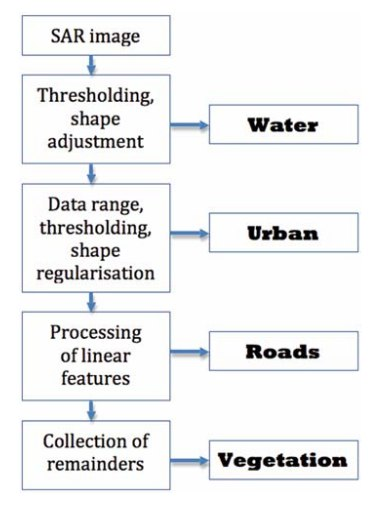
\includegraphics[width=0.35\linewidth]{Figures/ProcessingSteps.jpg}
	\label{Fig:ProcessingSteps}
\end{figure}

\begin{itemize}
    \item Autores:~\cite{dell2010rapid}
    \item Data de publicação: Mar. 2010
    \item Dataset
    \begin{itemize}
        \item Fonte: COSMO/SkyMed image of the Italian Space Agency and the Italian Civil Protection Department and TerraSAR-X image (courtesy of DLR).
        \item Região analisada: Chengdu outskirts and town of Luojiang.
    \end{itemize}
    \item Pré-processamento: pre-scaling of the image to a pixel size of 5 m is performed, according to the considerations expressed in (Pesaresi et al. 2007). The second step consists of a threshold operation over the computed occurrence map.
    \item Redução de dimensionalidade:
    \item Estruturas de dados: Texture.
    \item Técnica utilizada: Threshold and boundary regularization.
    \item Técnicas de visualização dos dados: The original COSMO/SkyMed image crop is shown. Red overlay on the original SAR image.
    \item Validação dos resultados: By inspection of the Google Earth image of the area.
    \item Foco do artigo: Urban area extraction and road map.
    \item Desafios e trabalhos futuros: Criteria for a suitable, automatic choice of the threshold value are under investigation. Small clusters of buildings sometimes may not be detected as urban areas and result in the production of false positives for the class “wood”. The model for roads is a series of linear segments, thus curvilinear roads have to be piecewise approximated, with a consequent loss of accuracy and possibly also completeness. This is a problem especially in higher relief areas where bends are frequent. A curvilinear model for roads should be integrated into the extraction algorithm if this is to be really complete. The trade-off between precision and speed of execution should not however be forgotten.
\end{itemize}

\newpage

\section*{Using Texture from High Resolution TerraSAR-X Images for Tropical forest mapping}

Tropical forests play an important role in improving the overall carbon footprint. Forests are a major carbon sink in the world.

The launch of TerraSAR-X satellite operating in X band ($\lambda$ = 3cm) with a metric spatial resolution in 2007, looks promising for the observation of tropical forests. 
Indeed, observations with smaller wavelength allow finer spatial resolutions. 
This feature provides access to textural information at scales of few meters, which was not accessible before with the previously existing SAR satellite.

The textural analysis has been widely studied with optical images (available since many years already) due to their high spatial resolution. 
Studies on textural analysis of SAR images were also performed, but mainly with airborne SAR data because of their identical spatial resolution to optical remote sensing data. 
In general, the textural analysis improves the precision of the vegetation type classifications [2], [3], [4], [5]. 
However, studies have shown a correlation between texture parameters and biomass with SAR data [6] or optical data [7].
Other studies have shown that the textural analysis could contribute directly to improve biomass estimation in the particular contexts such as mangroves in French Guiana, with optical data [8] , or a forest near Hong Kong, with SAR data [9].

The most common methods of textural analysis are based on the characterization of the co-occurrence matrix of gray levels (denoted GLCM) and retrieve Haralick parameters from it [10]. 
Some works have been done on the potential of radar data for classification of tropical forests in British and  Dutch Guiana [11]. 
These data were acquired by various airborne sensors in (X, C, L, and P) band during SAREX campaign in 1992. 
Methods based on the analysis of the backscattering coefficient, polarimetric indices and texture parameters of Haralick were evaluated. Texture analysis on the acquired images in X-band and C-band with the finest resolution of (6 m) was found to be the most suitable for classification, allowing the discrimination of 8 classes, 6 different forests types. 
And values of the backscattering coefficient data acquired in L-band, P and texture parameters calculated from data at high resolution X-band and C band give good performance in terms of classification of primary forests. 
Some other studies have been done using wavelet transform analysis and generalized Gaussian to characterize texture [12].

Texture is the spatial distribution (statistics) of gray levels [10].
Haralick parameters are estimated from a matrix of coocurrence of gray levels (GLCM), calculated from a grayscale image. 
Various parameters have been defined [10] to characterize the GLCM matrix; they correspond to the second order statistics of the original image. 
Among the 14 texture parameters introduced by Haralick, 1973, the six most used parameters are: Entropy, Contrast, Correlation, Energy, homogeneity. 
Haralick parameters depends on; filtering, logarithmic scale, gray level quantization, the size of the sliding window (w), the distance (d) and the analysis direction.

The retained algorithm of classification is the SVM (Support Vector Machine), as it allows taking into account numerous parameters, which can be heterogeneous with respect to their physical dimension. 
Past studies have shown that the SVM classification method is well suited to polarimetric radar data for vegetation classification [13].

The selection of the best Haralick parameters is based on the iterative feature selection method; Greedy Forward [13]. 
It can select the best suitable parameters and eliminates redundancy. 
Since the accuracy assessment statistics are biased in the case of a pixel-by-pixel classification.

In order to understand how we can differentiate between the different vegetation cover inside our image, the results were conducted successively over 3 different analyses: 
~i) Mean Vs Stdv of different forest plantation plots, 
~ii) classification based on color composite result, 
~iii) classification and post classification of 14 forest plantation classes including primary forest and riparian forest.

\begin{itemize}
    \item Autores:~\cite{benelcadi2014using}
    \item Data de publicação: Nov. 2014
    \item Dataset
    \begin{itemize}
        \item Fonte: High resolution Spotlight TerraSAR-X image (HS) operating in X band.
        \item Tempo de coleta: 28th September 2013.
        \item Volume dos dados: The TerraSAR-X image used in this case is an intensity single polarization HH image in HS300 mode with an incidence angle of $52^0$. The image size is $6.72 \times 7.95 km^2$ with a pixel size of 0.8m after orthorectification. 
        \item Região analisada: Forest of Brazil in Mato Grosso state in Fazenda Sao Nicolau.
    \end{itemize}
    \item Estruturas de dados: Texture and matrix of coocurrence of gray levels (GLCM).
    \item Técnica utilizada: Analysis of Haralick textural parameters, a second order statistic parameters computed in a certain direction with a distance (d) and window size (w). The retained algorithm of classification is SVM (Support Vector Machine as it allows taking into account numerous parameters, which can be heterogeneous with respect to their physical dimension.
    \item Técnicas de visualização dos dados: TerraSAR-X intensity image HH. Pléiade multispectral image. Color Composite (R: Energy
d4w15, G: Energy d8w31, B: SAR Intensity).
    \item Validação dos resultados: Ground truth data contained in the TerraSAR-X image. Confusion matrix is the assessment of the relationship between ground truth plots and post classification plots.
    \item Foco do artigo: Classification of tropical forest plantation of native species.
    \item Desafios e trabalhos futuros: It is not obvious to distinguish between the different plantation plots. And the only homogeneous information we can get from this region is about the leaf tree density. The integration of the post classification process inside the iterative feature selection method is still under development.
\end{itemize}

\newpage

\section*{Texture Fusion and Feature Selection Applied to SAR Imagery}

In the interpretation of synthetic aperture radar (SAR) images, texture [16] provides important information, in addition to image gray levels or the backscatter values alone. 
Several studies have shown that classification based on texture features can improve the accuracy of the interpretation [1], [2], [12], [17]. 
A large number of approaches for computation of image texture has been proposed in the literature. 
Some studies have compared the performance of different methods [2], [18] for SAR image analysis, but we are not aware of any study which has combined texture features derived from different models and then applied feature selection to find the optimal feature combination for a given classification task.

In this paper, we investigate the performance of texture features derived from the gray-level co-occurrence matrix [6], features based on local statistics, fractal features [11], and features derived from a log-normal random field model [4] for land-use classification of ERS-1 SAR images.

The co-occurrence texture features are based on gray-level spatial dependencies [6]. 
A co-occurrence matrix, computed in a local window, contains the relative frequencies of all pairwise combinations of backscatter values at a certain distance d and direction within the window. 
From this matrix, a number of features can be computed.

We compute the following texture features from the co-occurrence matrix: angular second moment (ASM), contrast (CONT), entropy (ENT), cluster shade (CLSH), inertia (INER), and inverse difference moment (IDM). 
These features are among the most commonly used co-occurrence features.

Prior to the computation of the co-occurrence matrix, the number of gray levels in the image needs to be reduced to a small number to get reliable estimates of the relative frequencies when texture is computed in a small window.
In this study, histogram equalization is first applied to the images to produce an image with gray levels which span the entire 8-bit range of pixel values, followed by a quantization into $N_g = 8$ gray levels.

Based on local statistics, the following features are computed: power-to-mean ratio, skewness, kurtosis, contrast [15] and homogeneity [15].

Many natural textured surfaces can be described as a fractal surface. 
The key parameter describing a fractal surface is its fractal dimension.
Several methods for computation of the fractal dimension of a surface exist.
The most common methods are the variation method [3], the e-blanket method [13], and the box-counting method [11]. 
In previous comparative studies [8] of the performance of these three methods, the variation method was found to have the smallest variance, indicating the best stability.

Several studies have shown that the fractal dimension alone does not capture all the textural properties (see, e.g., [11]). 
Another measure, called lacunarity, is often used in addition to the fractal dimension. 
The lacunarity value is small when texture is fine and it is large when the texture is coarse. 
An estimate of lacunarity can be derived from the box counting algorithm [11].

\begin{itemize}
    \item Autores:~\cite{solberg1997texture}
    \item Data de publicação: Mar 1997.
    \item Dataset
    \begin{itemize}
        \item Fonte: ERS- 1 SAR images.
        \item Tempo de coleta: fall of 1991.
        \item Volume dos dados: The size of the training areas was typically 4000 pixels per class for each image.
        \item Região analisada: Kjeller, Norway.
    \end{itemize}
    \item Estruturas de dados: Texture features derived from the gray-level co-occurrence matrix.
    \item Técnica utilizada: Feature selection methodology and discriminant analysis are applied to find the optimal combination of texture features. Following Frankot and Chellappa [4], we will model the SAR image using a multiplicative autoregressive random field (MAR). We can use either a nonparametric classifier, like the K -Nearest Neighbor classifier. Whitney’s algorithm for feature selection will be used [19].
    \item Técnicas de visualização dos dados: ERS-1 SAR subimages.
    \item Validação dos resultados: A comparison between the classification performance of the GLCM features, the local-statistics features, and features from the lognormal random field model is provided.
    \item Foco do artigo: A five-class classification problem was considered, consisting of the following common ground cover classes: water, urban areas, forests, and two classes of agricultural fields (plowed and unplowed).
\end{itemize}

\newpage

\section*{\textcolor{VioletRed4}{Textural Processing of Multi-Polarization SAR for Agricultural Crop Classification}}

The objective of these (second-order) statistical approaches (GLMC, GLDV and NGLDM) is to translate visual texture properties into quantitative descriptors in a manner that they can be used to discriminate relevant land features using additional image processing  techniques.

Tonal values in a synthetic aperture radar (SAR) image represent point measurements of the backscattering coefficient and are related to the radar wavelength and the elements within the scene that are interacting with the signal over a single pixel area. 
Texture, or the intrinsic spatial variability of SAR tone is recognized as an important interpretive tool for discriminating different land-cover and land-use types. 
A texture field within a SAR image is described as homogeneous if the spatial arrangement of pixel values are more homogeneous (as a unit) within than between texture fields [1]. 
In response to the need for extracting information based on the spatial arrangement of digital image data, numerous texture algorithms have been  developed based on structural approaches, Fourier power spectra, first-order statistics, second-order statistics, texture spectrum and spectral texture pattern matching. 
In studies comparing statistical texture measures, second-order gray-level co-occurrence statistical techniques tended to be superior to other statistical methods for capturing the textural content of an image [1].
Second-order statistical approaches [2], [3], [4] make use of gray-level probability density functions, which are generally computed as the conditional joint probability of pairs of pixel gray levels in a local area  of the image.

The GLCM is a two-dimensional array that provides the conditional joint probabilities of all pairwise combinations of pixels within a defined computation window [2].
The co-occurrence of gray values represents the probability of any two pairs of gray values occurring at a user-defined interpixel sampling distance and orientation. 
The texture statistics generated from the GLCM represent a single spatial measure of the image texture. 
These statistics are characterized as point estimates since each statistic provides a single measure of the distribution of gray-level pairs within the GLCM. 
Texture features (angular second moment, correlation and mean) based on GLCMs were generated by defining the following three input parameters: 
~(i) window size for which the co-occurrence matrix was generated; 
~(ii) interpixel sampling distance; and 
~(iii) direction for pixel co-occurrence within the sampling window [5].

The mean and correlation texture features derived from the GLCM provided the highest classification results. 
Results indicate that although texture features provide improved classification accuracy, the differences between the various texture features tested are generally small. 
Texture features derived from multi-polarimetric SAR data and integrated with optical data should provide sufficient discriminatory power when subjected to appropriate classification algorithms for identifying agricultural crops and crop conditions.  

\begin{itemize}
    \item Autores:~\cite{treitz1996textural}
    \item Data de publicação:  May 1996.
    \item Dataset
    \begin{itemize}
        \item Fonte: Airborne C-Band (5.3 GHz) SAR data with HH and HV polarizations.
        \item Tempo de coleta: July 10, 1990.
        \item Região analisada: Oxford County in southern Ontario Canada.
    \end{itemize}
    \item Estruturas de dados: Texture.
    \item Técnica utilizada: In this study, three techniques for generating texture statistics are examined: the Gray-Level CO-occurrence Matrix (GLCM), the Gray-Level Difference Vector (GLDV) and the Neighboring Gray-Level Dependence Matrix (NGLDM). Texture features generated from the GLCM, GLDV and NGLDM are classified individually using a k-Nearest Neighbor (k-NN) supervised classifier.
    \item Validação dos resultados: validation accuracy assessments.
    \item Foco do artigo: Agricultural crop classification and mapping.
\end{itemize}

\newpage

\section*{\textcolor{VioletRed4}{Contribution of textural information from TerraSAR-X image for forest mapping}}

Since 2007, radar sensors like Radarsat-2 or Terrasar-X offer high spatial resolution acquisition (about 1m), well suited to the patchwork parcels of European landscape, allowing their use on temperate regions.
Such resolution allows to access to textural information which was not possible with previous existing sensors such as ERS, ASAR with almost 25m of spatial resolutions.

This site contains 4 major land use areas (plantation area, service area, riparian area, and dense forest area).
We focus on 6 land cover classes: dense forest, riparian forest, bare and herbaceous soil, heterogeneous plantation with large row spacing, mono-plantation of teck with large row spacing and dense plantation of heterogeneous species.

Studies based on Fourier-based textural ordination (FOTO) analysis on optical images have shown very interesting results in biomass forest mapping [4].
The method consists in deriving the radial spectrum of the 2-D Fourier transform over a sliding window. 
Then, the radial spectrum is averaged over all directions.

For each selected wavelet, corresponding to a high pass filter, the resulting statistical distribution over a local neighborhood is assumed to follow a generalized Gaussian function.

Haralick attributes are extracted from the gray level co-ocurrence matrix (GLCM) [6].
Among the 14 textural attributes introduced by Haralick [6], eight different Haralick parameters have been retained: energy, entropy, correlation, homogeneity, contrast, mean, variance and dissimilarity.

For each of the 3 three methods, the same $50 \times 50$ window size have been retained.

\begin{itemize}
    \item Autores:~\cite{cazals2015contribution}
    \item Data de publicação: Nov. 2015
    \item Dataset
    \begin{itemize}
        \item Fonte: TerraSAR-X image.
        \item Tempo de coleta: 2013/09/28.
        \item Volume dos dados: The Terrasar-X image used for Sao Nicolau Fazenda site is an intensity single polarization HH acquisition in experimental mode High Resolution Spotlight 300 MHz.
        \item Região analisada: The study site is a forest plantation located in Brazil, in Mato Grosso state. Fazenda Sao Nicolau.
    \end{itemize}
    \item Estruturas de dados: Texture.
    \item Técnica utilizada: Three textural analysis methods have been compared : Fourier transform, wavelet transform and Haralick textural attributes. Their contribution for classification is assessed by their performance through the SVM algorithm.
    \item Técnicas de visualização dos dados: Textural information and TerraSAR-X image in mode High Resolution Spotlight.
    \item Validação dos resultados: Overall accuracy.
    \item Foco do artigo: This study evaluates the potential of High Resolution Spotlight TerraSAR-X image for forest type discrimination.
    \item Desafios e trabalhos futuros: Additional studies have to be made over different study sites to draw more general conclusions.
\end{itemize}

\newpage

\section*{\textcolor{VioletRed4}{Discriminating urban environments using multiscale texture and multiple SAR images}}

The characterization of urban environments by means of satellite data is becoming increasingly challenging because of the available ground spatial resolution of the sensors. 
However, a very high resolution is not always the solution to data interpretation problems. 
In fact, scales of urban features may be very different, and even for classification purposes they depend on the level of land cover/land use that one is seeking to discriminate (Woodcock and Strahler 1987). 
It is thus of paramount importance to find the best combination of data sets, feature manipulation techniques and interpretation/classification procedures for a given scale of interest.

In parallel, more recent work is trying to exploit the information in Synthetic Aperture Radar (SAR) images at the current coarse resolution, as provided by ERS, RADARSAT-1 and ENVISAT satellites as well as the Shuttle Imaging Radar missions (from SRL-1 to SRTM). 
Radar data are known to be affected by problems associated with the coarseness of their spatial resolution and the side-looking nature of the sensor. 
There are, however, a number of satellites with SAR sensors planned to be operative in the next few years with fine-resolution radar, from RADARSAT-2 to TerraSAR-X to the Cosmo/SkyMed constellation, while orientation-dependent problems may be overcome by combining different views of the same area (Dell’Acqua et al. 2003); their use become increasingly common with the new sensors and their short (less than 12 hours) revisit times.

However, one of the most interesting aspects of SAR data is that they provide information about scatterers in an area, and this has been used for many applications in the field of urban subsidence monitoring by differential interferometry (Ferretti et al. 2000). 
This information is also important to discriminate among different parts of the same urban areas by recognizing different scattering patterns. 
This approach has been proposed in Dell’Acqua and Gamba (2003), where single date and multi-temporal ERS data have been analyzed to detect the city center, residential areas and the outer sparsely built zones. 
The idea is based on the use of co-occurrence matrix texture measures. 
A similar method has been proposed in Dekker (2001) using other textures for the same purpose. 
This work is aimed at further investigation in the same field, that is the possibility of using different textures and/or different scales to improve the classification results.

As our problem is mainly to define which are the most useful textures for urban environment discrimination, we are mostly concerned with the use of the scale factor
in classification and interpretation algorithms. 
Among them, in Townshend and Justice (1988), the Fourier transform has been used to investigate the spatial frequency content and therefore the scale of an image. 
A similar approach has been proposed more recently by Chen and Blong (2003), but using a wavelet decomposition. 
The authors show that there is a function of the change in the statistics of the wavelet coefficients that has a maximum in correspondence with the scale of the features in the image. 
The methodology is quicker than Fourier transform, but also less accurate, due to the logarithmic spatial resolution levels of the wavelet transform. 
A precise analysis of the scales for different classes in the same scene has been proposed by Marceau et al. (1994). 
The authors presume that the window width giving the minimal variance in the neighborhood of each pixel for the largest number of bands may be used as the scale of the class to which the pixel belongs. 
It was found that, even for the same class, there are differences in the recognized scale, and this suggests the complexity of capturing this value. 
The approach is similar to that of Woodcock and Strahler (1987), as the neighborhood is used to compute local scale information through gray level variance, but it generalizes it, calling for a multi-scale analysis. 
The need for multiple scales suggested different approaches. 
Pesaresi and Benediktsson (2001) extracted spatial features referring to very different scales using morphological operators. 
An alternative approach has been proposed by Hay et al. (2001), who do not use  a series of images acquired at discrete scales, but rather use one single image at fine spatial resolution to capture the objects that emerge at their characteristic scale.

In practice, HDI computes how much the clusters of training samples referring to different classes overlap in the multidimensional feature space, and no assumption outside of the range of values in the training set is made.

\begin{itemize}
    \item Autores:~\cite{dell2006discriminating}
    \item Data de publicação: Feb. 2007
    \item Dataset
    \begin{itemize}
        \item Fonte: The data come from the ASAR sensor on board the ENVISAT satellite, from ERS-1/2 and from RADARSAT-1.
        \item Tempo de coleta: 13 August 1992
        \item Volume dos dados:
        \item Região analisada: Urban area of Pavia, Northern Italy.
    \end{itemize}
    \item Pré-processamento: As the data sets from ERS and ENVISAT have different spatial  resolution than the RADARSAT-1 fine beam images, two copies of the same ground truth were provided, at 12.5 m and 7 m ground resolution, and all the SAR data, possibly after slant-to-ground range conversion, were co-registered to one of these two reference maps.
    \item Redução de dimensionalidade: We prefer a feature extraction procedure based on the Histogram Distance Index (HDI) as a mean to detect the best feature subset. After this step, we are left with the most important textural features at different scales for the given data analysis problem, used as input to the classifier.
    \item Estruturas de dados: Texture.
    \item Técnica utilizada: Co-occurrence algorithm and the fuzzy ARTMAP classifier was applied to a set of four textures (mean, variance, dissimilarity and entropy). The analysis was performed by varying only one parameter at a time, and evaluating the classification results in terms of overall accuracy (OA) and mean class producer’s accuracy (MPA).
    \item Técnicas de visualização dos dados: Samples of SAR images, ground truth, classification maps for different SAR images and textural features.
    \item Validação dos resultados: For the purpose of data analysis, a ground truth was built by visual interpretation of a very fine resolution optical satellite image of the same area, an IKONOS-2 panchromatic image. Hints for interpretation and for characterizing past dates came from the corresponding sector of the Technical Regional Map, which is a raster map with 50 cm resolution, based on aerial photogrammetric flights in the early 1990s.
    \item Foco do artigo: Improve the characterization of an urban environment using multiscale textural features extracted from satellite SAR data.
    \item Desafios e trabalhos futuros: Our future work will focus on a further refinement of the procedure, aimed at extracting the boundaries of the urban areas with higher precision. We are also considering a different ground truth, more related to land use mapping. A future step will be to validate this new map. Finally, it is clearly necessary to prove the usefulness of this procedure in view of its application to more urban test sites, exploiting the experience we have gained on our data set.
\end{itemize}

\newpage

\section*{\textcolor{VioletRed4}{Efficient Texture Analysis of SAR Imagery}}

Texture is an important visual cue, used by both man and machine in describing and assessing object surfaces.
The texture of an object surface depends on a number of factors, such as the spatial relation between primitive texture elements, their scale, and/or orientation. 
The spatial and scale properties of texture have made it an important attribute in the analysis of remotely sensed images, where different surfaces such as those of rocks, sea-ice, sea-water, vegetation, urban areas, etc. can be characterized by distinct textural features.

Different methods have been proposed for the analysis of image texture. 
Popular methods include those based on the gray-level co-occurrence matrix (GLCM) [11], Markov random fields (MRFs) [16], Gabor wavelets [14], [17], tree-structured wavelets [6], wavelet packets [21], sum-difference histograms, etc. 
See [22] for comparative performance of general texture analysis schemes. 
For analysis of remotely sensed images, the GLCM-based methods are the most predominant, e.g., see [2], [13], [19], [23], and [24].
In [25], the performance of various second-order statistical textural features was evaluated for classification of sea-ice radar imagery. 
Clausi [8], [9] compared the performance of GLCM, MRF, and Gabor features in classifying SAR sea-ice imagery. 
He found that the GLCM produced the overall best results in terms of classification accuracy, followed by the Gabor features. 
However, the GLCM features were found to be more sensitive to texture boundaries as compared to MRF. 
Carr and Miranda [5] compared the semivariogram and the GLCM on classification of two terrestrial SAR images acquired from six different spectral bands. 
The GLCM provided a better classification accuracy for optical images, while the semivariogram did better on microwave images. 
Thus, there is no general agreement on an overall best analysis method—one that outperforms all the others on various tasks, such as classification [3], retrieval [17], or segmentation [14]. 
Combining the different analysis methods for improved robustness has been suggested [8].

In general, the major focus of research in texture analysis has been on the construction of texture representations that will provide the most discrimination ability.
One underlying fact about the various methods, however, is that texture analysis is a very time consuming process. 
This is mainly due to the need to consider multiple orientations and multiple scales in order to accurately capture the textural characteristics of a given surface.

Texture analysis is inherently computationally intensive. 
Automated analysis of object texture usually requires point-by-point computations on the object surface. 
These operations typically involve some kind of image filtering, using neighboring points in a chosen window around the point under consideration.
For SAR imagery, texture analysis usually requires a consideration of both the micro- and macrotextural structures in the image. 
The use of textural contexts [24] is the basic approach to dealing with such global and local properties of texture. 
Another source of difficulty is the sheer volume of data involved. Some SAR image analysis problems involve high-rate, high-quality multichannel and multitemporal images, with image sizes running into millions of pixels.

For the GLCM, basic methods used in handling computation include using reduced gray-levels [7], [9], [24], reduced size of the subimages [7], or choosing only a few features [13], [24]. 
Holmes et al. [13] proposed the use of image slicing (basically gray-level quantization) to improve the speed of analysis. 
In [3], computation was reduced by applying texture analysis methods on reduced versions of the original image, based on the multiresolution pyramid. 
Soh and Tsatsoulis [24] used an average of the GLCM matrices over different scales and orientations to reduce computation. 
In [2] and [7], the symmetry and the sparseness of the GLCM were used to avoid unnecessary computations.


\begin{itemize}
    \item Autores:~\cite{kandaswamy2005efficient}
    \item Data de publicação: Sept. 2005
    \item Dataset
    \begin{itemize}
        \item Fonte: The first is a set of nine images taken from the Brodatz texture album [4], a popular texture set used in general research in texture analysis. The second dataset is a collection of seven Advanced Synthetic Aperture Radar (ASAR) images, taken from cold regions with a diversity of texture characteristics, such as various types of sea-ice, sea-water, snow, etc. All the SAR images in the dataset were obtained from the European Space Agency.
        \item Tempo de coleta: 2002-2003
        \item Região analisada: The SAR images were taken in some locations in Finland and Antarctica.
    \end{itemize}
    \item Pré-processamento: Rather than using the entire image data for the analysis, we use an approximation of the image.
    \item Redução de dimensionalidade: We selected $512 \times 512$ sub-image areas from the original source image. For each image, we selected ten $64 \times 64$ texture areas that represent the general texture class in the image. Each source image used characterizes one specific texture class. No two source images contain visually similar textures.
    \item Estruturas de dados: Texture.
    \item Técnica utilizada: Motivated by the statistical occupancy model, we introduce the notion of patch re-occurrences. Using the re-occurrences, we propose the use of approximate textural features in analysis of SAR images. We describe how the proposed approximate features can be extracted for two popular texture analysis methods - the gray-level co-occurrence matrix and Gabor wavelets. Approximate textural features on SAR images.
    \item Técnicas de visualização dos dados: Boxes representing the different classes within SAR images.
    \item Validação dos resultados: Nine test images from the Brodatz Texture Album. Verification of the ground truths.
    \item Foco do artigo: supervised and unsupervised classification (using k-means and distance measure) of SAR image textures.
    \item Desafios e trabalhos futuros: In this work, we have assumed a simple uniform distribution. Given the generalized Rayleigh model for SAR image [15], one interesting future work will be to further refine the choice of parameters in our approach, based on the model of SAR images. Further, given that the approximate image could contain structural/spatial information relating the image patches, it might be possible to exploit this for further improvement in robustness and efficiency.
\end{itemize}

\newpage

\section*{\textcolor{VioletRed4}{Textural Information in SAR Images}}

A multiplicative model was used to relate the image variance for a given land-use category to the individual variances associated with image speckle and target texture. 
Speckle was treated as a random process governed by signal fading and was considered to be statistically independent of the textural variations associated with the spatial variations of the scattering properties of visually "uniform" distributed targets.

The first-order statistics of the fading and texture random variables describe their probability density functions (pdf). 
The second-order fading and texture statistics (such as the auto-correlation function) describe the relationships between a pixel and its neighbors. 
In both first- and second-order statistics there is a need to separate the fading.

The first-order texture variance for both the intensity and the square-root intensity images is directly proportional to the square of the normalized image standard deviation. 
If the scene categories have similar mean values, then there will be no difference in the classification performance of the texture
variance and image variance.

Second-order statistics based on the gray-level co-occurrence matrix are simpler to compute. 
Thus, second-order spatial statistics give superior results to tonal and first-order statistics in the classification of land-use on Seasat radar images.

\begin{itemize}
    \item Autores:~\cite{ulaby1986textural}
    \item Data de publicação: Mar. 1986
    \item Dataset
    \begin{itemize}
        \item Fonte: SIR-A SAR data and Seasat SAR data.
        \item Região analisada: Northeastern Oklahoma and North and South America.
    \end{itemize}
    \item Estruturas de dados: Texture. 
    \item Técnica utilizada: Multiplicative model. First-order: Intensity Image, Square-Root Intensity Image and Amplitude Image. Second-Order Image Statistics: Speckle Auto-correlation Function of an Intensity Image, Speckle Auto-correlation Function of a Square-Root Intensity Image, Texture Auto-correlation of a Digital Intensity Image and Texture Auto-correlation of a Digital Square-Root Intensity Image. The second-order gray-level co-occurrence (GLC): Contrast and inverse moment. Maximum-likelihood techniques.
    \item Técnicas de visualização dos dados: Photographs of forested areas typical of the five forest categories considered in this study, Geographic locations, radar texture.
    \item Validação dos resultados: Dataset.
    \item Foco do artigo: Classification of five land-use categories: water, forest, pasture, urban, and cultivated.
\end{itemize}

\newpage

\section*{\textcolor{VioletRed4}{Texture Analysis and Classification of ERS SAR Images for Map Updating of Urban Areas in The Netherlands}}

In single-band and single-polarized synthetic aperture radar (SAR) image classification, texture holds useful information.
Among them were histogram measures, wavelet energy, fractal dimension, lacunarity, and semivariograms.

The area can be characterized as a well-planned dispersed urban area with residential areas, industry, greenhouses, pasture, arable land, and some forest.
The study was done on the basis of non-parametric separability measures and classification techniques because most texture distributions were not normal.

Automatic or semiautomatic map updating using remote sensing images is an important area of research. 
A growing amount of remote sensing information is available today from different types of sensors. 
A certain level of automation can speed-up the map updating process considerably.

Sensors such as the ERS-1/2, Envisat, and Radarsat-1 deliver images with a resolution of about 25 m, which is appropriate to update 1 : 250 000 maps (100 image pixels per map centimeter). 
Most are single band and single polarized, which limits the information to intensity and texture. 
Only Envisat is dual polarized.
In tandem configuration, i.e., one-day repeat pass, the coherence can be used for map updating [7], [23].
Future SAR satellites will be dual or fully polarized (e.g., Radarsat-2, Cosmo/SkyMed, and TerraSAR) and can supply polarimetric information for map updating using polarimetric decomposition techniques [6], [10], [13]. 
Besides, they will have a better resolution ( 5 m), which will result in different textures [28].

In map updating using ERS-1, one of the most interesting questions is which texture measures can best be used for discriminating different types of (urban) land cover, in addition to the image intensity.

Histogram Measures: The most common class of texture measures is the class of histogram measures. 
Well known are the mean Euclidean distance, variance, skew, kurtosis, entropy, and energy [11], [27].
Another histogram texture measure is the weighted-rank fill ratio, which is defined by Novak et al.[19].

Wavelet Energy Measures: The wavelet transform is a multiresolution decomposition. 
It can be interpreted as the inverse Fourier transforms of the set of logarithmically divided frequency bins [5]. 
Each decomposition level consists of four components: a high-pass, a low-pass, a horizontal, and a vertical component.
Entropy and energy (6) and (7) of the different components are a measure of texture. 
The energy was used because it gave better classification results [16].
Bellagente et al. [2] compared different wavelet transforms for texture characterization, and concluded that the Daubechies wavelet with four coefficients (DAUB4) resulted in the highest classification accuracy.

Fractal Dimension: Fractal-based descriptions have been used successfully in texture analysis and segmentation of images [21]. 
Descriptors can be derived from the definition of the mass of a fractal surface within a window [15], [21].
The lacunarity is, as is the mass, a function of the observation scale or window size $r$.
Several methods exist to estimate the fractal dimension [1], [19], [21], [24]. 
Stewart et al. [24] concluded that the power spectral-density method is the most accurate.
Another method for estimating the fractal dimension using the wavelet transform is given by Espinal et al. [29].
An advantage of the method of Espinal et al. is that it enables estimating multiple dimensions in the case of multi-fractal surfaces. 
On the other hand, this method is possibly correlated with the wavelet energy measures because there is a direct connection between the fractal dimension and wavelet energy.

Lacunarity: Another aspect of fractal surfaces is the lacunarity [15]; see also (9). 
Several methods exist to estimate the lacunarity [9], [17], [22], but a disadvantage of most methods is that they can only be applied to binary images (i.e., images with a depth of one bit). 
Therefore, images with a larger depth have to be threshold first, introducing an extra parameter. 

Semivariogram: The semivariogram was chosen as an alternative for the well-known gray-level co-occurrence family of features because it gave better results on SAR data [4].

To study the separability of features, in this paper the texture measures, a distance must be chosen that corresponds to the type of classifier that is used. 
For instance, for the Bayes quadratic classifier, the Bhattacharyya distance is most appropriate because both assume normal-distributed variables. 
In case of the NN classifier in the previous section, a non-parametric separability measure is more appropriate. 
Fukunaga [14] gives different separability measures based on the within-class and between-class scatter matrices.

\begin{itemize}
    \item Autores:~\cite{dekker2003texture}
    \item Data de publicação: Sept. 2003.
    \item Dataset
    \begin{itemize}
        \item Fonte: European Remote Sensing Satellite 1 (ERS-1) SAR image. ERS-1 operates in the C-band and is Vertical–Vertical (VV) polarized.
        \item Tempo de coleta: The image was acquired June 23, 1995 (ERS-1 orbit 20601, frame 1035), and was logarithmically scaled.
        \item Volume dos dados: The size of the subimage is $3209 \times 3273$ pixels ($64.2 \times 65.5$ km).
        \item Região analisada: Rotterdam and The Hague in The Netherlands.
    \end{itemize}
    \item Granularidade da análise: Based on existing land-cover and physical properties with respect to radar, five classes were defined: urban, industry/greenhouses, forest, water, and other. 
    \item Estruturas de dados: Texture.
    \item Técnica utilizada: Previous results were presented in [32] and [33]. Nonparametric classifier is the nearest neighbor ( NN) classifier. Based on an extensive study of literature, a set of promising texture measures was selected.
    \item Técnicas de visualização dos dados: ERS-1 SAR subimage. Generalized VMap1 of topografische. Results in map of classification techniques. Histograms of the sample areas of the ERS-1 SAR image.
    \item Validação dos resultados: The map of the Randstad Holland was obtained from VMap1 data, which was produced by the Topografische Dienst Nederland (TDN).
    \item Foco do artigo: Texture Analysis and Classification of Urban Areas in The Netherlands.
    \item Desafios e trabalhos futuros: An interesting question is if future high-resolution radar satellites as the ones mentioned in the Introduction provide more land-cover texture to improve the classification accuracy. Unfortunately, this question cannot be answered yet, unless data from airborne radar sensors are used.
\end{itemize}

\newpage

\section*{\textcolor{VioletRed4}{Texture Analysis of SAR Sea Ice Imagery Using Gray Level Co-Occurrence Matrices}}

We computed the texture matrix representations of these sample contexts and used a supervised Bayesian classifier to evaluate how well the texture matrices could describe and recognize the textural contexts.
The texture matrix used was the gray-level co-occurrence matrix (GLCM).

We performed a set of experiments in which we systematically varied these parameters and studied how the variations affected GLCM standard texture descriptors for SAR sea ice images. 
From these experiments, we concluded which quantization levels and displacement and orientation values are best for representing sea ice texture in SAR.
We concluded which texture matrix representation is best at separating sea ice texture types in SAR imagery.

Statistical texture analysis is important in SAR sea ice imagery research since it allows better representation and segmentation of sea ice regions, compared to analysis based on intrinsic gray levels only. 
It has been shown that the inclusion of texture as a descriptor can improve the classification of sea ice and the description of sea ice deformations [38], [56], [63].

Our work is the first one to evaluate all possible textural representation parameters and to make specific recommendations about the representation of sea ice texture in SAR imagery.

We used ten textural features in our study: Energy, Contrast, Correlation, Homogeneity, Entropy, Auto-correlation, Dissimilarity, Cluster Shade, Cluster Prominence, Maximum Probability.
Note that energy is also popularly known as angular second moment [30].

Haralick et al. [35] illustrated the applications of textural features based on GLCM on three different kinds of image data: photomicrographs of different kinds of sandstones [60], panchromatic aerial photographs of land-use categories, and earth resources technology satellite (ERTS) multi-spectral imagery containing land-used categories.

We showed that 
~1) 256-level representation is not necessary, 
~2) eight-level representation is undesirable, and 
~3) 64-level representation is efficient and sufficient.
Second, we compared three different implementations of co-occurrence matrices: MDMO, ODMO, and ODOO.
Third, we presented a Bayes classifier that yielded $99.19\%$ of training set and $94.17\%$ of test set classification accuracies into seven classes on 240 samples.
This indicates that 
~1) sea ice textural contexts can be successfully represented and used to classify different types of SAR sea ice imagery and 
~2) sea ice textural contexts can be successfully represented using GLCM-based features.

\begin{itemize}
    \item Autores:~\cite{soh1999texture}
    \item Data de publicação: Mar 1999 
    \item Dataset
    \begin{itemize}
        \item Fonte: 100-m ERS-1 synthetic aperture radar (SAR) imagery.
        \item Tempo de coleta: 
        Class 1 -- March 27, 1992, at $73.466^0$ N and $156.19^0$ E. 
        Class 2 -- February 7, 1993, at $58.54^0$ N and $163.63^0$ W.
        Class 3 -- September 8, 1993, at $77.35^0$ N and $145.79^0$ W.
        Class 4 -- July 12, 1993, at $72.26^0$ N and $160.47^0$ W.
        Class 5 -- February 1, 1994 at $72.06^0$ N and $176.39^0$ W.
        Class 6 - November 17, 1993, at $72.27^0$ N and $154.75^0$ W.
        Class 7 -- March 17, 1992, at $72.85^0$ N and $143.83^0$ W.
        \item Volume dos dados: We analyzed over 2000 ERS-1 SAR low-resolution images.
        \item Região analisada: Bering, the Beaufort, and the Chukchi seas.
    \end{itemize}
    \item Redução de dimensionalidade: We computed the texture matrix representations of these sample contexts and used a supervised Bayesian classifier to evaluate how well the texture matrices could describe and recognize the textural contexts. The texture matrix used was the gray-level co-occurrence matrix (GLCM).
    \item Estruturas de dados: Texture.
    \item Técnica utilizada: We used gray-level co-occurrence matrices (GLCM) to quantitatively evaluate textural parameters and representations and to determine which parameter values and representations are best for mapping sea ice texture. We conducted experiments on the quantization levels of the image and the displacement  and orientation values of the GLCM by examining the effects textural descriptors such as entropy have in the representation of different sea ice textures. In addition, we developed three GLCM implementations and evaluated them by a supervised Bayesian classifier on sea ice textural contexts.
    \item Técnicas de visualização dos dados: Images of regions represented by textures.
    \item Validação dos resultados: Human visual inspection.
    \item Foco do artigo: In this paper, we present a set of experiments on textural parameters and representations and a quantitative evaluation of these experiments, which shows which textural parameter values and texture representations are best for describing sea ice in synthetic aperture radar (SAR) imagery. 
    \item Desafios e trabalhos futuros: Our future work in this research includes applying sea ice textural contexts to refine classification based on spectral and surface textural information.
\end{itemize}

\newpage

\section*{\textcolor{VioletRed4}{Texture-based characterization of urban environments on satellite SAR images}}

We investigate the use of co-occurrence texture measures to provide information on different building densities inside a town structure. 
We try to improve the pixel-by-pixel classification of an urban area by considering texture measures as a means for block analysis and classification.

So, there is an interest in the analysis of radar images of urban areas, given also SAR all-weather capabilities and, therefore, its usefulness for disaster monitoring. 
However, in urban areas, where objects tend to cluster and show almost no regular structure, the problems of radar imaging have long prevented SAR from being useful for urban characterization.

Fuzzy ARTMAP structure that has already shown superior performance in classifying very complex environments, like urban ones [6]. 
The neural classifier may be applied directly to the ERS images, one at a time or as a multi-temporal sequence [4], retrieving the built-up area with a sufficiently high precision.

In order to choose the best feature set for the classification, we considered six test areas ($25 \times 25$ pixels wide), two for each of the considered building density class. 
To provide a quantitative assessment of texture measures ability to discriminate the urban environments, we use in the test areas the histogram density index (HDI) to compare textural information [12].
The more they are different, the higher the HDI, and the more useful is this feature to discriminate between the classes the test areas belong to. 
Since we have six test areas, we have 17 combinations: the final HDI is the mean among all these comparisons and represents to what extent a feature could be helpful to recognize urban environments by their building density.

\begin{itemize}
    \item Autores:~\cite{dell2003texture}
    \item Data de publicação: Jan 2003.
    \item Dataset
    \begin{itemize}
        \item Fonte: The dataset used in this research corresponds to subsamples of six ERS-1 images.
        \item Tempo de coleta: Acquired between 1992 and 1994.
        \item Região analisada: Urban and suburban area around the town of Pavia, Northern Italy.
    \end{itemize}
    \item Estruturas de dados: Texture.
    \item Técnica utilizada: We considered textural features computed by means of the co-occurrence matrix [11] and applied our neurofuzzy classifier to many different textural combinations, computed with different window width. We computed the eight texture measures: Contrast, correlation, dissimilarity, entropy, mean, homogeneity, second moment, variance.
    \item Técnicas de visualização dos dados: Different kinds of ground truth available for the urban study area (Pavia, Northern Italy). 
    ~(a) pixel-by-pixel seven-classes ground truth. 
    ~(b) Ground truth for building density, computed starting by the previous image, where the “city center” is in white, “residential areas” in gray, and “suburban areas” in light gray. 
    ~(c) Same three environments, as they are recognized by manual interpretation of very high resolution satellite data (other light gray tones represent vegetation and water respectively, ignored in this application).
    Building density mapped from multi-temporal ERS classification.
    Fuzzy ARTMAP building density classifications.
    Some examples of differences between the ground truth and the classification results.
    \item Validação dos resultados: The map was extracted from the Regional Technical Map of the Lombardia Region, suitably resampled to match the SAR data. The same map may also be used to delineate a detailed ground truth of the test area by means of manual interpretation. Accuracy values.
    \item Foco do artigo: We try to improve the pixel-by-pixel classification of an urban area by considering texture measures as a means for block analysis and classification. 
\end{itemize}

\newpage

\section*{\textcolor{VioletRed4}{Using SAR images to delineate ocean oil slicks with a texture-classifying neural network algorithm (TCNNA)}}

SAR is therefore useful for detecting surfactant layers produced by floating oil.
Ocean slicks are a subset of ocean features detected in SAR data. 
They are areas of distinctly contrasting brightness against the radar backscatter produced by wind-generated ripples.
Slicks are contiguous areas in which Bragg scattering at a wavelength scale of $\sim 0.01–0.10$ m is suppressed by layers of oil (Alpers and Espedal, 2004; Hu et al., 2008), biological surfactants, or floating vegetation (Huehnerfuss et al., 1983).

\begin{itemize}
    \item Autores:~\cite{garcia2009using}
    \item Data de publicação: Apr. 2010.
    \item Dataset
    \begin{itemize}
        \item Fonte: Through data-sharing agreements with the National Aeronautical and Space Administration (NASA) and support from the Alaska Satellite Facility (ASF), a collection of almost 700 RADARSAT-1 images.
        \item Região analisada: Gulf of Mexico.
    \end{itemize}
    \item Pré-processamento: Quality control of the data required a series of steps. 
    After converting analog SAR signals from RADARSAT-1 to binary SAR data, the ASF Data Center provided the SAR data in Committee on Earth Observation Satellites (CEOS) level one SKY telemetry format (Gens and Logan, 2003). 
    Converter tool software provided by ASF was then used to construct GeoTIFF images from the raw binary SAR data. 
    However, a set of fixed oil platforms was used to verify and fix the georectification.
    \item Redução de dimensionalidade:
    \item Estruturas de dados: Texture.
    \item Técnica utilizada: Texture-classifying neural network algorithm.
    \item Técnicas de visualização dos dados: Subset of a RADARSAT-1 image. Georectified eight-bit SAR image.
    \item Validação dos resultados: Dataset.
    \item Foco do artigo: We developed a texture-classifying neural network algorithm (TCNNA), which processes SAR data from a wide selection of beam modes, to extract these patterns from SAR imagery in a semisupervised procedure. Our approach uses a combination of edge-detection filters, descriptors of texture, collection information (e.g., beam mode), and environmental data, which are processed with a neural network. Examples of pattern extraction for detecting natural oil seeps in the Gulf of Mexico are provided.
\end{itemize}

\newpage

\section*{\textcolor{VioletRed4}{Land cover mapping of the Mekong Delta to support natural resource management with multi-temporal Sentinel-1A synthetic aperture radar imagery}}

The method can be divided into three steps: 
~(i) pre-processing, 
~(ii) generation of texture images using GLCM measure, 
~(iii) comparison of classification accuracy (single-date versus multi-temporal, single-date versus multi-temporal with texture, multi-temporal versus multi-temporal with texture) and the calculation of the Z-test statistic. 

\begin{itemize}
	\item Autores~\cite{Ngo2020land}
	\item Data de publicação: Jan. 2020
	\item Dataset
	\begin{itemize}
		\item Fonte: Sentinel-1A C-band SAR images collected by the European Space Agency (ESA). 
		\item Tempo de coleta:  Acquired in 2016,
		\item Volume dos dados: Twenty-one SAR images.
		\item Região analisada: Mekong Delta.
	\end{itemize}
	\item Pré-processamento: The SAR images were pre-processed to produce Grey Level Co-occurrence Matrix (GLCM) texture images. Radiometric calibration.
	\item Estruturas de dados: Texture.
	\item Técnica utilizada: Support Vector Machines (SVM) and Random Forest (RF).
	\item Técnicas de visualização dos dados: Study area location in map, land cover classes in optical images and SAR backscatter coefficient images extraction at VH polarization. Result of classification in map.
	\item Validação dos resultados: Dataset. overall accuracy and Kappa coefficient. 
	\item Foco do artigo: Characterise urban, forest, aquaculture, and rice paddy field for the three input image sets. 
	\item Desafios e trabalhos futuros: One of the greatest challenges in our study area was distinguishing between paddy fields and shrimp farming. 
	Another source of error which resulted in misclassification was between shrimp farms and paddy fields, as they all include different combinations of vegetation, water and bare soil. 
	Other sources of error common to SAR classification in general are due to the small variations of the incidence angle of Sentinel-1A satellite and ground truth errors contributed the mapping results. 
	The most problematic issue in the study area for classification was the confusion between rice crop and shrimp farming. To eliminate this, potentially additional extraction methods based on phenological characteristics of rice crop could be used to distinguish rice crop from shrimp farming class.
\end{itemize}

\newpage

\section*{\textcolor{VioletRed4}{Nome do Artigo}}

\begin{itemize}
	\item Autores:
	\item Data de publicação:
	\item Dataset
	\begin{itemize}
		\item Fonte:
		\item Tempo de coleta:
		\item Volume dos dados:
		\item Região analisada:
	\end{itemize}
	\item Granularidade da análise:
	\item Pré-processamento:
	\item Redução de dimensionalidade:
	\item Estruturas de dados:
	\item Técnica utilizada:
	\item Técnicas de visualização dos dados:
	\item Validação dos resultados:
	\item Foco do artigo:
	\item Desafios e trabalhos futuros:
\end{itemize}

\newpage


\bibliographystyle{agsm}
\bibliography{references.bib}


\end{document}